% =============================================================================
% Section 6.2: Gained Experience
% =============================================================================

\section{Gained Experience}
\label{sec:experience}

The NexaLearn project provided hands-on experience across a wide range of software engineering disciplines. This section summarises the key skills and knowledge acquired during the design, implementation, and testing phases. Figure~\ref{fig:skills-radar} presents a self-assessment of proficiency gained across eight competency areas.

\begin{figure}[H]
  \centering
  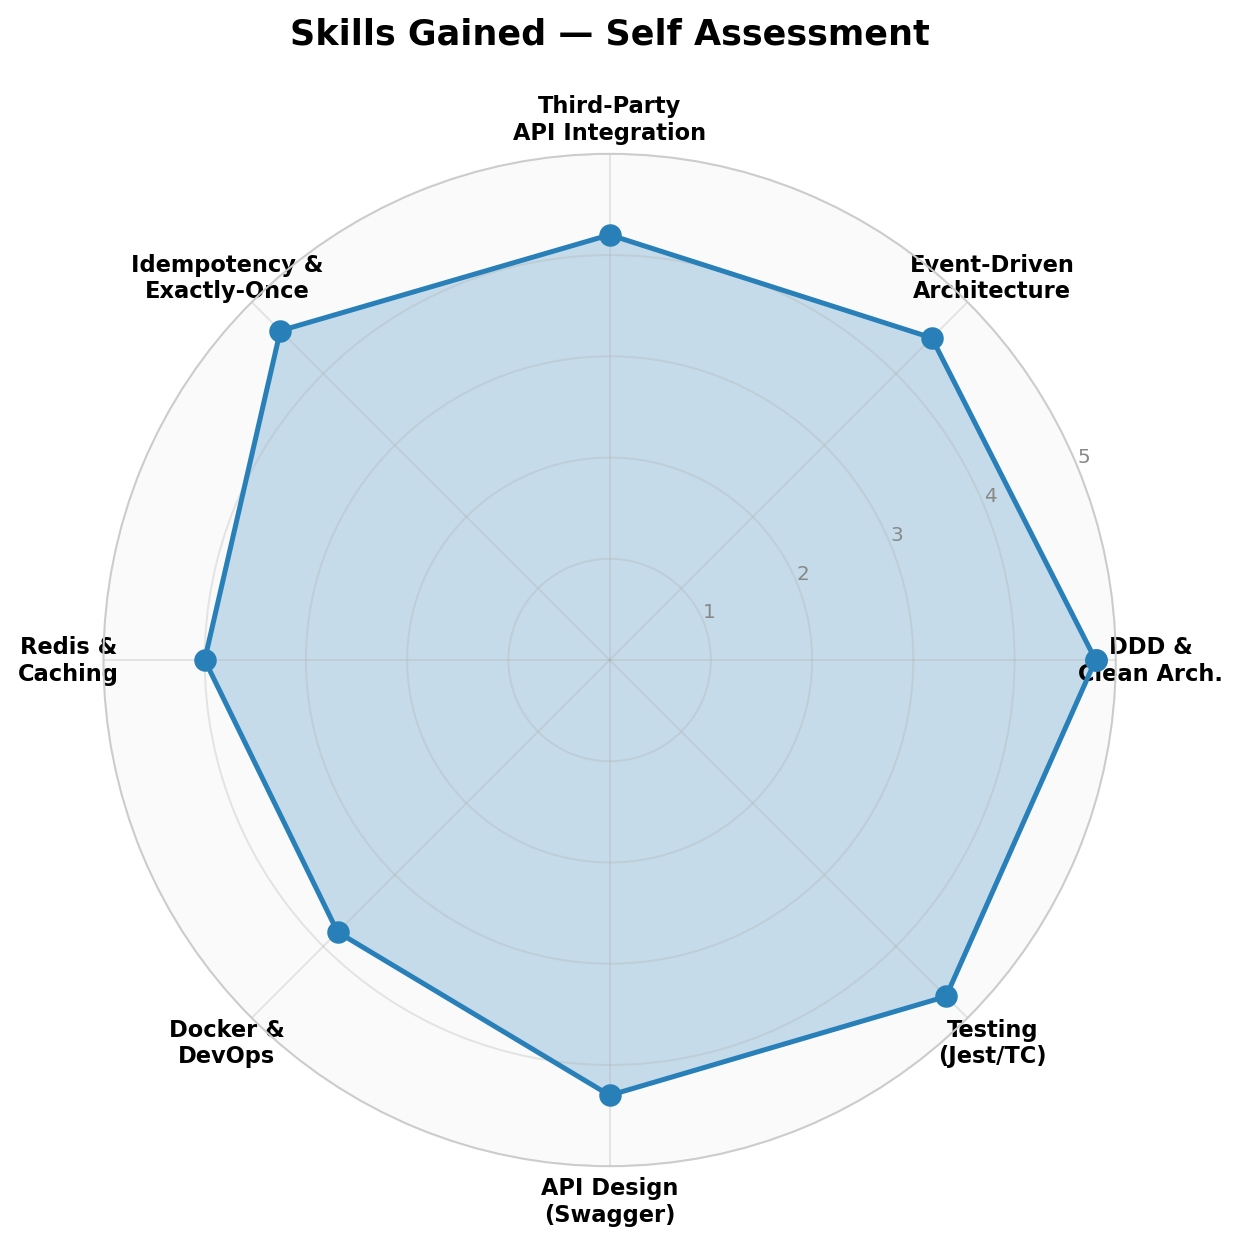
\includegraphics[width=0.65\textwidth]{images/skills_radar.png}
  \caption{Skills gained during the NexaLearn project, self-assessed across eight dimensions on a 1--5 scale.}\label{fig:skills-radar}
\end{figure}

\subsection{Domain-Driven Design in Practice}

Prior to this project, DDD was understood primarily through literature---Evans' blue book~\cite{evans2003ddd}, Vernon's red book, and online resources. Implementing fifteen bounded contexts in a real codebase revealed the practical nuances that textbooks do not capture: how to handle shared kernel relationships between closely related contexts (e.g., Assessment and AI Pipeline share the \texttt{Quiz} concept but diverge in their representation); how to size aggregates so that consistency boundaries are neither too large (performance degradation) nor too small (invariant leakage); and how to evolve the ubiquitous language when the team discovers that a term means different things in different contexts.

The decision to enforce DDD boundaries through NestJS module encapsulation and TypeScript \texttt{private} access modifiers on aggregate methods was validated repeatedly. When a developer inadvertently attempted to mutate an aggregate's internal state from an application service, the TypeScript compiler rejected the code at compile time rather than at runtime.

\subsection{Event-Driven Architecture and Reliable Messaging}

Designing the transactional outbox pattern from scratch---rather than adopting an existing library like \texttt{@nestjs/cqrs} or \texttt{pg-boss}---provided deep insight into the subtleties of reliable event delivery. The key lessons learned include:

\begin{itemize}
  \item \textbf{Polling frequency vs. latency trade-off.} The outbox poller runs every 500 ms by default. Reducing this to 100 ms decreases event delivery latency but increases database load. A configurable polling interval with adaptive backpressure (slowing down when the outbox table is empty) would be the ideal design.
  \item \textbf{\texttt{SELECT FOR UPDATE SKIP LOCKED}} is essential for concurrent outbox consumers. Without it, two poller instances can claim the same event, leading to duplicate processing.
  \item \textbf{Event schema evolution.} The outbox stores event payloads as JSON. Adding a new field to an event requires backward-compatible readers, which is straightforward with TypeScript's optional properties but requires discipline in the event handler implementations.
\end{itemize}

\subsection{Third-Party API Integration}

The project integrated with four external services, each presenting unique integration challenges:

\begin{itemize}
  \item \textbf{Stripe.} The Stripe API is well-documented, but webhook signature verification, idempotency key management, and event versioning require careful handling. The project implemented a custom \texttt{StripeWebhookGuard} that verifies the \texttt{Stripe-Signature} header using the raw body and the webhook secret, mirroring Stripe SDK best practices.
  \item \textbf{Mux.} Mux's asset lifecycle is more complex than a simple upload--transcode--deliver pipeline. Understanding the state machine---\texttt{uploaded}, \texttt{preparing}, \texttt{ready}, \texttt{errored}, and the separate MP4 rendition state---was essential for correctly sequencing the AI pipeline.
  \item \textbf{AWS S3.} Presigned URL generation for direct browser-to-S3 uploads eliminated the need for the server to proxy file uploads, reducing bandwidth costs and latency. The \texttt{@aws-sdk/client-s3} SDK's \texttt{PutObjectCommand} with \texttt{PresignedPost} was used for this purpose.
  \item \textbf{Resend (Email).} Transactional email delivery (verification, enrollment confirmation, password reset) was outsourced to Resend. The integration was straightforward, but templating email content for both HTML and plain-text formats required a templating strategy using Handlebars.
\end{itemize}

\subsection{Designing for Idempotency and Exactly-Once Semantics}

Perhaps the most transferable skill gained was the systematic approach to idempotency. Every external-facing endpoint and event handler in NexaLearn is designed to be safe to retry. The patterns employed---optimistic concurrency control, projection event ledger, Redis atomic operations, and domain-level state machines---are broadly applicable to any distributed system. The key insight was that idempotency is a cross-cutting concern that must be considered at the architecture level, not retrofitted into individual handlers.

\subsection{Infrastructure and DevOps}

The project provided practical experience with Docker containerisation, Docker Compose for local development, and Nginx as a reverse proxy for serving the application and static assets. The CI pipeline configured in GitHub Actions---running tests in parallel shards with Testcontainer-backed databases, generating coverage reports, and building the Docker image---mirrors the setup used in production-grade open-source projects.

Swagger/OpenAPI documentation is auto-generated from the NestJS controllers using the \texttt{@nestjs/swagger} package. Every endpoint is annotated with \texttt{@ApiTags}, \texttt{@ApiOperation}, and \texttt{@ApiResponse} decorators, producing a live documentation page at \texttt{/api/docs} that allows interactive API exploration. This proved invaluable during integration testing and would serve as the primary reference for frontend developers building on top of the API.

\subsection{Team Collaboration and Version Control}

The project was developed using Git with a feature-branch workflow. Pull requests were reviewed for architectural consistency, adherence to DDD principles, test coverage, and code style. The experience of maintaining a consistent ubiquitous language across fifteen bounded contexts reinforced the importance of clear communication and documentation in a multi-module codebase.
